\chapter{Opis teoretyczny}
\label{cha:opis_teor}

\section{Gra 3 osobowa}
\label{sec:3_gra}

\paragraph{O jakiej grze mówimy}

W niniejszej pracy będziemy skupiali się na grze 3-osobowej.Będziemy rozpatrywać tylko przypadki w których koalicja dwóch graczy wygrywa. Nie bierzemy pod uwagę sytuacji w których współpraca ze sobą wszystkich graczy mogłaby przynieść najlepsze korzyści. W tabelce wypłat rozważanej gry nie może pojawić się punkt równowagi wynikający ze strategii czystych. W rozważane przez nas grze celem gracza nie jest zdobycie jak największego zysku, lecz osiągnięcie jak największej liczby wygranych. Osoba znajdująca się poza koalicją przegrywa i wszyscy gracze mają taką samą wagę wyboru.

Będziemy rozważali dwa przypadki: zależnej i niezależnej rozgrywki. Przez rozgrywkę niezależną rozumiem grę w której wynik partii w żaden sposób nie zależy od innych prowadzonych gier. Grę w okręgu opisuję jako rozgrywkę zależną, gdyż wybór dokonany lokalnie przez gracza wpływa na wyniki wyniki sąsiednich gier lokalnych. W pierwszej części skupimy się na partiach niezależnych, a następnie wykonamy symulacje gier ze sobą powiązanych. W grach zależnych każdy gracz będzie rozgrywał partie z dwoma innymi graczami siedzącymi po obu jego stronach, będzie to przypominało grę w okręgu gdzie każdy z graczy może wybrać czy wstępuje w koalicję z swoim partnerem po prawej czy lewej stronie. W takiej sytuacji nie będzie możliwe granie z oboma partnerami. Będziemy w końcu zmuszeni wybrać z kim trzymamy stałą koalicję, a kogo odrzucimy. Wykluczamy możliwość jakiejkolwiek komunikacji między graczami poza obserwowaniem ich poprzednich zagrań. Model ten z pewnością będzie dużo bardziej dynamiczny, gdyż częstotliwości wybierania sojuszy będzie musiała zmienić zachowanie sojuszników naszych partnerów.

\section{Model gry}
W niniejszej pracy będziemy potrzebowali dwóch modeli gier. Pierwszym z nich będzie model gry 3-osobowej niezależnej( brak powiązań z innymi grami). Należy to postrzegać jako izolowaną od otoczenia grę 3 zawodników. Zacznijmy od nazwania graczy odpowiednio $G_0$, $G_1$, $G_2$ (gracz pierwszy, drugi, trzeci). Każdy z nich posiada prawdopodobieństwo zagrania na gracza o wyższym indeksie (zapętlamy dla trzeciego gracza) $p_i$. Prawdopodobieństwo zagrania na gracza o niższym indeksie (zapętlamy dla pierwszego gracza) wynosi $1 - p_i$ i nie musi być przechowywane, ponieważ możemy to w łatwy sposób wyliczyć. Ponadto są one dostępne tylko dla graczy, których opisują. Żaden z zawodników nie ma dostępu do prawdopodobieństw innych graczy, lecz każdy ma dostęp do statystyki gry na którą składa się:
\begin{itemize}
\item $liczba_{partii}$ liczba rozegranych w grze partii
\item $nast_i$ ilość zagrań $G_i$ na gracza $G_{i+1}$, ilość zagrań na $G_{i-1}$ możemy wziąć z $liczba_{partii} - nast_i$
\end{itemize}
Drugi z modeli będzie się nieznacznie różnił. Będzie to gra n-osobowa składająca się z lokalnych gier 3-osobowych. Pozostała cześć modelu się nie zmienia.
{\color{red} UKŁAD}
\begin{figure}
	\centering
	\begin{tabular}{c|c}
	\subfloat[niezależny \label{fig:model_niezal}]{ 
		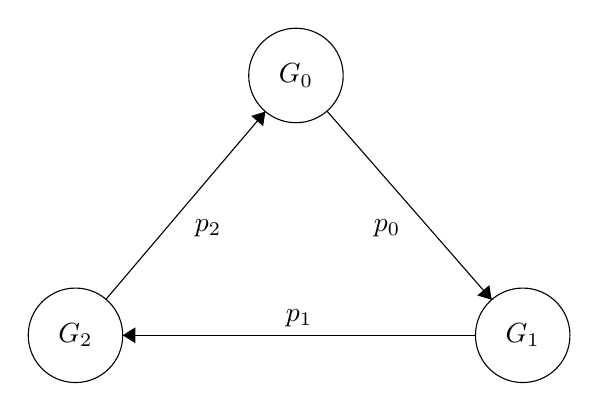
\begin{tikzpicture}[scale=0.2]
		\tikzstyle{every node}+=[inner sep=0pt]
		\draw [black] (40.6,-18.2) circle (3);
		\draw (40.6,-18.2) node {$G_0$};
		\draw [black] (55,-34.7) circle (3);
		\draw (55,-34.7) node {$G_1$};
		\draw [black] (26.6,-34.7) circle (3);
		\draw (26.6,-34.7) node {$G_2$};
		\draw [black] (42.57,-20.46) -- (53.03,-32.44);
		\fill [black] (53.03,-32.44) -- (52.88,-31.51) -- (52.12,-32.17);
		\draw (47.26,-27.9) node [left] {$p_0$};
		\draw [black] (52,-34.7) -- (29.6,-34.7);
		\fill [black] (29.6,-34.7) -- (30.4,-35.2) -- (30.4,-34.2);
		\draw (40.8,-34.2) node [above] {$p_1$};
		\draw [black] (28.54,-32.41) -- (38.66,-20.49);
		\fill [black] (38.66,-20.49) -- (37.76,-20.77) -- (38.52,-21.42);
		\draw (34.15,-27.89) node [right] {$p_2$};
		\end{tikzpicture}
	} &
	\subfloat[zależny \label{fig:model_zal}]{  
		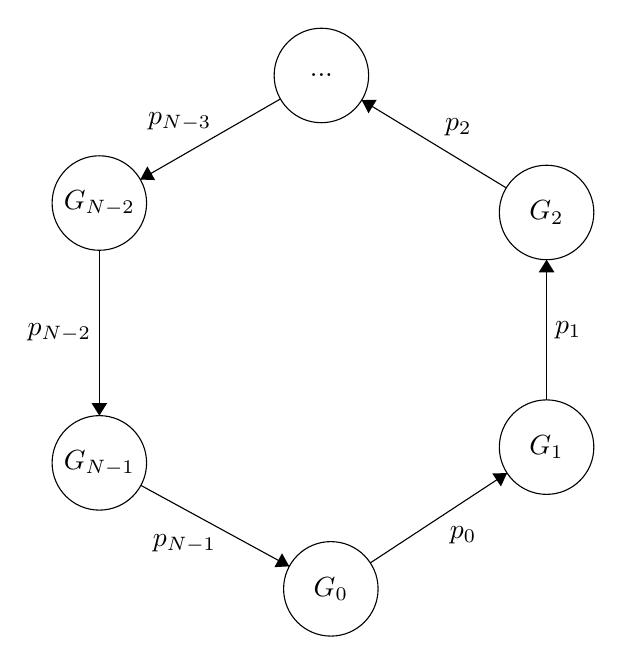
\begin{tikzpicture}[scale=0.2]
		\tikzstyle{every node}+=[inner sep=0pt]
		\draw [black] (38.2,-44.1) circle (3);
		\draw (38.2,-44.1) node {$G_0$};
		\draw [black] (51.9,-35.1) circle (3);
		\draw (51.9,-35.1) node {$G_1$};
		\draw [black] (23.5,-36.1) circle (3);
		\draw (23.5,-36.1) node {$G_{N-1}$};
		\draw [black] (51.9,-20.2) circle (3);
		\draw (51.9,-20.2) node {$G_2$};
		\draw [black] (23.5,-19.6) circle (3);
		\draw (23.5,-19.6) node {$G_{N-2}$};
		\draw [black] (37.6,-11.5) circle (3);
		\draw (37.6,-11.5) node {$...$};
		\draw [black] (40.71,-42.45) -- (49.39,-36.75);
		\fill [black] (49.39,-36.75) -- (48.45,-36.77) -- (49,-37.6);
		\draw (46.6,-40.1) node [below] {$p_0$};
		\draw [black] (26.14,-37.53) -- (35.56,-42.67);
		\fill [black] (35.56,-42.67) -- (35.1,-41.84) -- (34.62,-42.72);
		\draw (28.91,-40.6) node [below] {$p_{N-1}$};
		\draw [black] (23.5,-22.6) -- (23.5,-33.1);
		\fill [black] (23.5,-33.1) -- (24,-32.3) -- (23,-32.3);
		\draw (23,-27.85) node [left] {$p_{N-2}$};
		\draw [black] (51.9,-32.1) -- (51.9,-23.2);
		\fill [black] (51.9,-23.2) -- (51.4,-24) -- (52.4,-24);
		\draw (52.4,-27.65) node [right] {$p_1$};
		\draw [black] (49.34,-18.64) -- (40.16,-13.06);
		\fill [black] (40.16,-13.06) -- (40.59,-13.9) -- (41.11,-13.05);
		\draw (46.3,-15.35) node [above] {$p_2$};
		\draw [black] (35,-12.99) -- (26.1,-18.11);
		\fill [black] (26.1,-18.11) -- (27.04,-18.14) -- (26.55,-17.27);
		\draw (28.6,-15.05) node [above] {$p_{N-3}$};
		\end{tikzpicture}
	}
	\end{tabular}
\caption{Modele gry}
\label{fig:modele}
\end{figure}

Wszystkie zmiany prawdopodobieństwa muszą przejść funkcję ograniczającą, więcej o niej znajdziemy w sekcji \ref{sec:ograniczenie}. Jak uzyskać $\Delta p_i$ dowiemy się w dwóch następnych podrozdziałach.
\begin{equation} \label{eq:ograniczenie}
p_i = ogr( p_i + \Delta p_i)
\end{equation}
%---------------------------------------------------------------------------------------------------------------------------------------------------------------------

\section{Równania standardowe}
\label{sec:r_stand}
Podstawowym równaniem od którego wyjdziemy będzie równanie dla gracza o indeksie 0, pozostałe utworzymy analogicznie:
\begin{equation} \label{eq:poczatek}
\Delta p_0 = (1 - p_1) - p_2
\end{equation}
Dlaczego akurat to? Sposób rozumowania jest prosty. Człon $1 - p_1$ jest prawdopodobieństwem zagrania gracza 1 na gracza 0, więc prawdopodobieństwo zagrania gracza 0 na gracza 1 powinno z nim rosnąć. Co mogłoby zniechęcić gracza 0 do sympatyzowania z graczem 1? Sojusz między graczem 2 a 1? Zdecydowanie nie! Z tego właśnie powodu odejmujemy $p_2$, co ma pokazywać graczowi 0 że ma innego zawodnika, który wyciąga do niego rękę.

Następnym pytaniem jest: skąd mam wiedzieć z jakim prawdopodobieństwem gra mój przeciwnik? Nie masz wiedzieć. Z tego względu zdecydowałem się wprowadzić u zawodników statystykę zagrań przeciwników, pozwalającą obliczyć prawdopodobieństwo. Czy takie coś się sprawdzi? Tak i nie, w jednej z następnych sekcji \ref{sec:ograniczenie} omówimy bardziej szczegółowo niechciane zachowania z tego wynikające, ale na chwilę obecną przyjmijmy, że potrzebujemy dodatkowego parametru $\alpha$ przyjętego na poziomie $0.1$.

W poniższym równaniu $n_N$ oznacza liczbę partii zagranych przez następnego (z wyższym indeksem) gracza w kierunku jego następnego gracza. Analogicznie $n_P$ oznacza liczbę partii zagranych przez poprzedniego (z niższym indeksem) gracza w kierunku jego następnego gracza (czyli nas).
\begin{equation} \label{eq:stand}
\Delta p_i = \alpha \cdot (1 - \frac{n_N}{liczba_{partii}} - \frac{n_P}{liczba_{partii}})
\end{equation}

%---------------------------------------------------------------------------------------------------------------------------------------------------------------------

\section{Równania replikatorów}
\label{sec:r_repli}

OPISAĆ SPOSÓB WYPROWADZENIA OBYDWU!!! I CZYNNIK ZMNIEJSZAJĄCY NA KRAŃCACH !!!

\begin{equation} \label{eq:repli}
p_i += \alpha \cdot (p_i \cdot (1 - p_i)) \cdot (1 - \frac{n_R}{nr_{games}} - \frac{n_L}{nr_{games}})
\end{equation}

%---------------------------------------------------------------------------------------------------------------------------------------------------------------------

\section{Ograniczenie prawdopodobieństwa}
\label{sec:ograniczenie}
Jak zauważyliśmy powyższe równania w łatwy sposób mogą wyjść poza przedział $<0,1>$. Aby temu zapobiec każda inkrementacja prawdopodobieństwa musi być obłożona funkcją ograniczającą. Każde nowo obliczone prawdopodobieństwo podawane jest jako parametr do funkcji $ogr$, a dopiero jej rezultat jest przypisywany poszczególnym graczom. Zdecydowałem się użyć następującej funkcji:
\begin{displaymath}
ogr(p_i) = \left\{
\begin{array}{ll}
1 & \text{jeżeli } p_i > 1 \\
p_i & \text{jeżeli } 1 \geq p_i \geq 0 \\
0 & \text{jeżeli } p_i < 0
\end{array} 
\right\}
\end{displaymath}

Zapewne naszą uwagę przykuł także parametr $\alpha$ obecny w powyższych równaniach. W pierwszym z nich użycie go jest konieczne, gdyż w przeciwnym przypadku szacowanie prawdopodobieństwa innych doprowadziłoby to zawiązania trwałych koalicji już po pierwszej partii. N oznacza zagranie w stronę zawodnika z wyższym numerem, natomiast P z niższym. Zapętla to się dla pierwszego i ostatniego gracza. Zobaczmy przykład dla równania standardowego, prawdopodobieństwa początkowego $\frac{1}{2}$ i $\alpha = 1$ zakładając że:
\begin{align*}
Gracz_0 = N, Gracz_1 = P, Gracz_2 = N && Gracz_0 = N, Gracz_1 = P, Gracz_2 = P\\
\left\{
\begin{array}{ll}
\Delta p_0 = (1 - 0 - 1) =  0 & p_0=\frac{1}{2}\\
\Delta p_1 = (1 - 1 - 1) =  -1 & p_1= 0\\
\Delta p_2 = (1 - 1 - 0) =  0 & p_2=\frac{1}{2}\\
\end{array} 
\right\} &&
\left\{
\begin{array}{ll}
\Delta p_0 = (1 - 0 - \frac{1}{2}) =  0 & p_0=\frac{3}{4}\\
\Delta p_1 = (1 - \frac{1}{2} - 1) =  -\frac{1}{2} & p_1= 0\\
\Delta p_2 = (1 - 0 - \frac{1}{2}) =  \frac{1}{2} & p_2=\frac{3}{4}\\
\end{array}
\right\}
\end{align*}
Schemat po lewej przedstawia pierwszą partię, a po lewej drugą. Jak widzimy prowadzi to do bardzo szybkich zmian prawdopodobieństwa, co może praktycznie uniemożliwiać jakiekolwiek zmiany sojuszy. Co jednak z równaniami replikatorów? Czy również tam potrzebny będzie nam jakiś parametr zmniejszający dynamikę? Przecież zawierają one człon postaci $x(1-x)$, czy to nie wystarczy? Weźmy założenia z poprzedniego przykładu. Przeanalizujmy przykład: {\color{red} UKŁAD}
\begin{align*}
Gracz_0 = N, Gracz_1 = P, Gracz_2 = N \\
\left\{
\begin{array}{ll}
\Delta p_0 = \frac{1}{2} \cdot (1 - \frac{1}{2}) \cdot (1 - 0 - 1) =  0 & p_0=\frac{1}{2}\\
\Delta p_1 = \frac{1}{2} \cdot (1 - \frac{1}{2}) \cdot (1 - 1 - 1) =  0 & p_1= \frac{1}{4}\\
\Delta p_2 = \frac{1}{2} \cdot (1 - \frac{1}{2}) \cdot (1 - 0 - 1) =  0 & p_2=\frac{1}{2}\\
\end{array} 
\right\}
\\
Gracz_0 = N, Gracz_1 = P, Gracz_2 = P \\
\left\{
\begin{array}{ll}
\Delta p_0 = \frac{1}{2} \cdot (1 - \frac{1}{2}) \cdot (1 - 0 - \frac{1}{2}) = \frac{1}{8} & p_0=\frac{5}{8}\\
\Delta p_1 = \frac{1}{4} \cdot (1 - \frac{1}{4}) \cdot (1 - \frac{1}{2} - 1) = -\frac{1}{32} & p_1= \frac{7}{32}\\
\Delta p_2 = \frac{1}{2} \cdot (1 - \frac{1}{2}) \cdot (1 - 0 - \frac{1}{2}) = \frac{1}{8}  & p_2=\frac{5}{8}\\
\end{array}
\right\}
\end{align*}
Jak widzimy najszybsza zmiana zachodzi dla pierwszego gracza, który traci 25\% zaufania do gracza o wyższym indeksie. W kolejnej partii nie widzimy już tak dużych zmian. Czy jest to na tyle dużo, aby wprowadzać parametr mający spowalniać dynamikę zmian? Zanim odpowiem chciałbym poruszyć dwie kwestie. Zgadzam się że dynamika prawdopodobieństwa jest dla mnie akceptowalna(czyli wynosi do 10\%), ale tylko dla prawdopodobieństw które oddalają się od środka przedziału, a grę rozpoczynamy właśnie w nim. Drugą sprawą jest porównanie obu równań. Porównanie wyników, w które rekurencyjnie wkładamy czynnik wymnażający zmianę nie jest najłatwiejszą rzeczą do opisania. Ale czy człon $x(1-x)$ w równaniu replikatorów nie jest takim czynnikiem? Owszem jest, ale ... właśnie jego celem jest rozwiązanie problemu supersilnych, szybko tworzących się koalicji.

Postarajmy się teraz skupić na szczególnych przypadkach, gdy w obu osobnych grach żaden z graczy nie współpracował. Użyjemy równań standardowych, prawdopodobieństwo początkowe $\frac{1}{2}$ oraz $\alpha = 1$.

\begin{align*}
Gracz_0 = N, Gracz_1 = N, Gracz_2 = N && Gracz_0 = P, Gracz_1 = P, Gracz_2 = P \\
\left\{
\begin{array}{ll}
\Delta p_0 = (1 - 1 - 1) =  -1 & p_0=0\\
\Delta p_1 = (1 - 1 - 1) =  -1 & p_1= 0\\
\Delta p_2 = (1 - 1 - 1) =  -1 & p_2=0\\
\end{array} 
\right\} &&
\left\{
\begin{array}{ll}
\Delta p_0 = (1 - 0 - 0) =  1 & p_0= 1\\
\Delta p_1 = (1 - 0 - 0) =  1 & p_1= 1\\
\Delta p_2 = (1 - 0 - 0) =  1 & p_2= 1\\
\end{array}
\right\}
\end{align*}
Przypadek ten pokaże nam skutki braku ograniczenia w prawdopodobieństwie. Wiemy że teraz każdy z graczy wykona ruch przeciwny do poprzedniego co da nam w obu grach:
\begin{align*}
\left\{
\begin{array}{l}
\Delta p_0 = (1 - \frac{1}{2} - \frac{1}{2}) =  0 \\
\Delta p_1 = (1 - \frac{1}{2} - \frac{1}{2}) =  0 \\
\Delta p_2 = (1 - \frac{1}{2} - \frac{1}{2}) =  0 \\
\end{array} 
\right\}
\end{align*}
Brak wpływu na zmiany, gracze dokonują wyboru jak poprzednio.
\begin{align*}
Gracz_0 = P, Gracz_1 = P, Gracz_2 = P && Gracz_0 = N, Gracz_1 = N, Gracz_2 = N \\
\left\{
\begin{array}{ll}
\Delta p_0 = (1 - \frac{1}{3} - \frac{1}{3}) =  \frac{1}{3} & p_0= \frac{1}{3}\\
\Delta p_1 = (1 - \frac{1}{3} - \frac{1}{3}) =  \frac{1}{3} & p_1= \frac{1}{3}\\
\Delta p_2 = (1 - \frac{1}{3} - \frac{1}{3}) =  \frac{1}{3} & p_2= \frac{1}{3}\\
\end{array} 
\right\} &&
\left\{
\begin{array}{ll}
\Delta p_0 = (1 - \frac{2}{3} - \frac{2}{3}) =  -\frac{1}{3} & p_0= \frac{2}{3}\\
\Delta p_1 = (1 - \frac{2}{3} - \frac{2}{3}) =  -\frac{1}{3} & p_1= \frac{2}{3}\\
\Delta p_2 = (1 - \frac{2}{3} - \frac{2}{3}) =  -\frac{1}{3} & p_2= \frac{2}{3}\\
\end{array}
\right\}
\end{align*}
Wróciliśmy to punktu wyjścia, tylko tym razem wyjściowym prawdopodobieństwem chęci gry na gracza z większym indeksem jest $\frac{1}{3}$ dla gry przedstawionej po lewej stronie i $\frac{2}{3}$ dla gry po prawej? Nie do końca! W pamięci każdego z graczy jest liczba rozegranych partii ze swoimi rywalami co będzie prowadziło do niekoniecznie oczywistych zachowań, gdy przeanalizujemy ścieżki gier o wyborach z większym prawdopodobieństwie.
\begin{align*}
Gracz_0 = P, Gracz_1 = P, Gracz_2 = P && Gracz_0 = N, Gracz_1 = N, Gracz_2 = N \\
\left\{
\begin{array}{ll}
\Delta p_0 = (1 - \frac{1}{4} - \frac{1}{4}) =  \frac{1}{2} & p_0= \frac{5}{6}\\
\Delta p_1 = (1 - \frac{1}{4} - \frac{1}{4}) =  \frac{1}{2} & p_1= \frac{5}{6}\\
\Delta p_2 = (1 - \frac{1}{4} - \frac{1}{4}) =  \frac{1}{2} & p_2= \frac{5}{6}\\
\end{array} 
\right\} &&
\left\{
\begin{array}{ll}
\Delta p_0 = (1 - \frac{2}{5} - \frac{2}{5}) =  -\frac{1}{2} & p_0= \frac{1}{6}\\
\Delta p_1 = (1 - \frac{2}{5} - \frac{2}{5}) =  -\frac{1}{2} & p_1= \frac{1}{6}\\
\Delta p_2 = (1 - \frac{2}{5} - \frac{2}{5}) =  -\frac{1}{2} & p_2= \frac{1}{6}\\
\end{array}
\right\}
\end{align*}
Widzimy zmianę zachowania graczy spowodowaną sumą częstości gier przeciwników. Sytuacja takiej fluktuacji będzie się powtarzać, lecz z czasem będziemy tracić naszą pulę graczy z powodu czynnika prawdopodobieństwa. Teoretycznie mając do dyspozycji nieskończoną populację graczy oraz nieograniczony czas, istniałby przypadek nieskończonej ,,sinusoidy'' o zwiększającym się okresie. Sytuacja taka nie jest dla nas pożądana, co stanowi dodatkowy argument za użyciem parametru $\alpha < 1$ skutecznie niwelującego wystąpienie takich sytuacji.
